%\newcommand*{\SCRIPT}{}
\newcommand*{\BEAMER}{}

\ifdefined\SCRIPT
	\documentclass{article}
	\usepackage[a4paper, left=2.5cm, right=2cm, top=5.5cm, bottom=2.5cm]{geometry}
	\usepackage[noxcolor]{beamerarticle}
	\usepackage[ngerman]{babel}
	\usepackage[utf8]{inputenc}
	\usepackage{amsmath}
	\usepackage{amsthm}
	\usepackage{graphicx}
	\usepackage{pgfplots}
	\usepackage{tcolorbox}
	\usepackage{siunitx}
	\sisetup{locale = DE,
	per-mode=fraction}
	\usetikzlibrary{arrows,patterns}
	\usepackage{biblatex}
	\usepackage{xltabular}
	\addbibresource{Schallgeschwindigkeit.bib}
	\usepackage{scrlayer-scrpage}
	\pagestyle{scrheadings}
	\clearpairofpagestyles
	\ofoot{Seite \pagemark}
	\newcolumntype{C}[1]{>{\centering\arraybackslash}p{#1}}
	\DeclareNewLayer[%
	  background,% Hintergrundebene
	  width=\textwidth,% Größe und Position des Textbereichs
	  hoffset=2.5cm,
	  voffset=2.5cm,
	  align=tl,
	  contents={%
	  \sffamily
	    \setlength{\fboxsep}{2mm}% Abstand Box Text
	    \setlength{\fboxrule}{.5mm}% Dicke Linie
	    % vertikale Position korrigieren    
	    \vskip-\fboxsep\vskip-\fboxrule\vskip-\baselineskip
	    % horizontale Position korrigieren
	    \hspace{-\fboxsep}\hspace{-\fboxrule}%
	    \begin{tabularx}{\textwidth}{|>{\bfseries\Large}C{7cm}|X|X|}                                                       
	\hline
	\vspace{0em}
\includegraphics[scale=0.3]{logo2.png} & Name: & Datum: \\
	\hline
	
	\end{tabularx}
	    %\makebox[\layerwidth][l]{%
	    %  \fbox{\rule{0pt}{\layerheight}\rule{\layerwidth}{0pt}}% Rahmen
	    %}%
	  }
	]{frame}
	\AddLayersToPageStyle{@everystyle@}{frame}
\fi

\ifdefined\BEAMER
	\documentclass{beamer}
	\usepackage[ngerman]{babel}
	\usepackage[utf8]{inputenc}
	\usepackage{amsmath}
	\usepackage{amsthm}
	\usepackage{siunitx}
	\usepackage{graphicx}
	\usepackage{pgfplots}
	\sisetup{locale = DE,
	per-mode=fraction}
	\usetikzlibrary{arrows,patterns}
	% Lade Beamer Stile
	\usepackage{beamerthemesplit}
	\usepackage{tcolorbox}
	\usetheme{Rochester}
	\usecolortheme{crane}
\fi

\title{4. Unterrichtseinheit zur Dynamik}
\subtitle{Impuls und Kraftstoß}
\author{Heiko Schröter}
\date{\today}

\setbeamertemplate{enumerate item}{\alph{enumi})}

\begin{document}

\frame{\titlepage}

\frame
{
  \frametitle{Ziele für die heutige Unterrichtseinheit}
  \textbf{Impuls und Kraftstoß}
  \begin{itemize}
	\item Was versteht man unter einem Impuls?
	\item Wie ist der Kraftstoß definiert?
	\item Wann tritt eine Änderung des Impulses ein?
	\item Beispielaufgabe zum Stoß
	\item Übungsaufgaben
  \end{itemize}
}

\frame
{
  \frametitle{Die Bewegungsgröße (Impuls)}
\begin{block}{Impuls}
Unter der Bewegungsgröße bzw. dem Impuls $p$ eines Körpers versteht man das Produkt seiner Masse $m$ und seiner Geschwindigkeit $v$. Einheit: \si{\kilogram\meter\per\second}.
\begin{align*}
p=m\cdot v\quad\quad [p]=[m]\cdot[v]=\si{\kilogram}\cdot\si{\meter\per\second}=\si{\kilogram\meter\per\second}
\end{align*}
\end{block}
}

\frame
{
  \frametitle{Beispiel Impuls einer fallenden Kugel}
      \begin{figure}
	  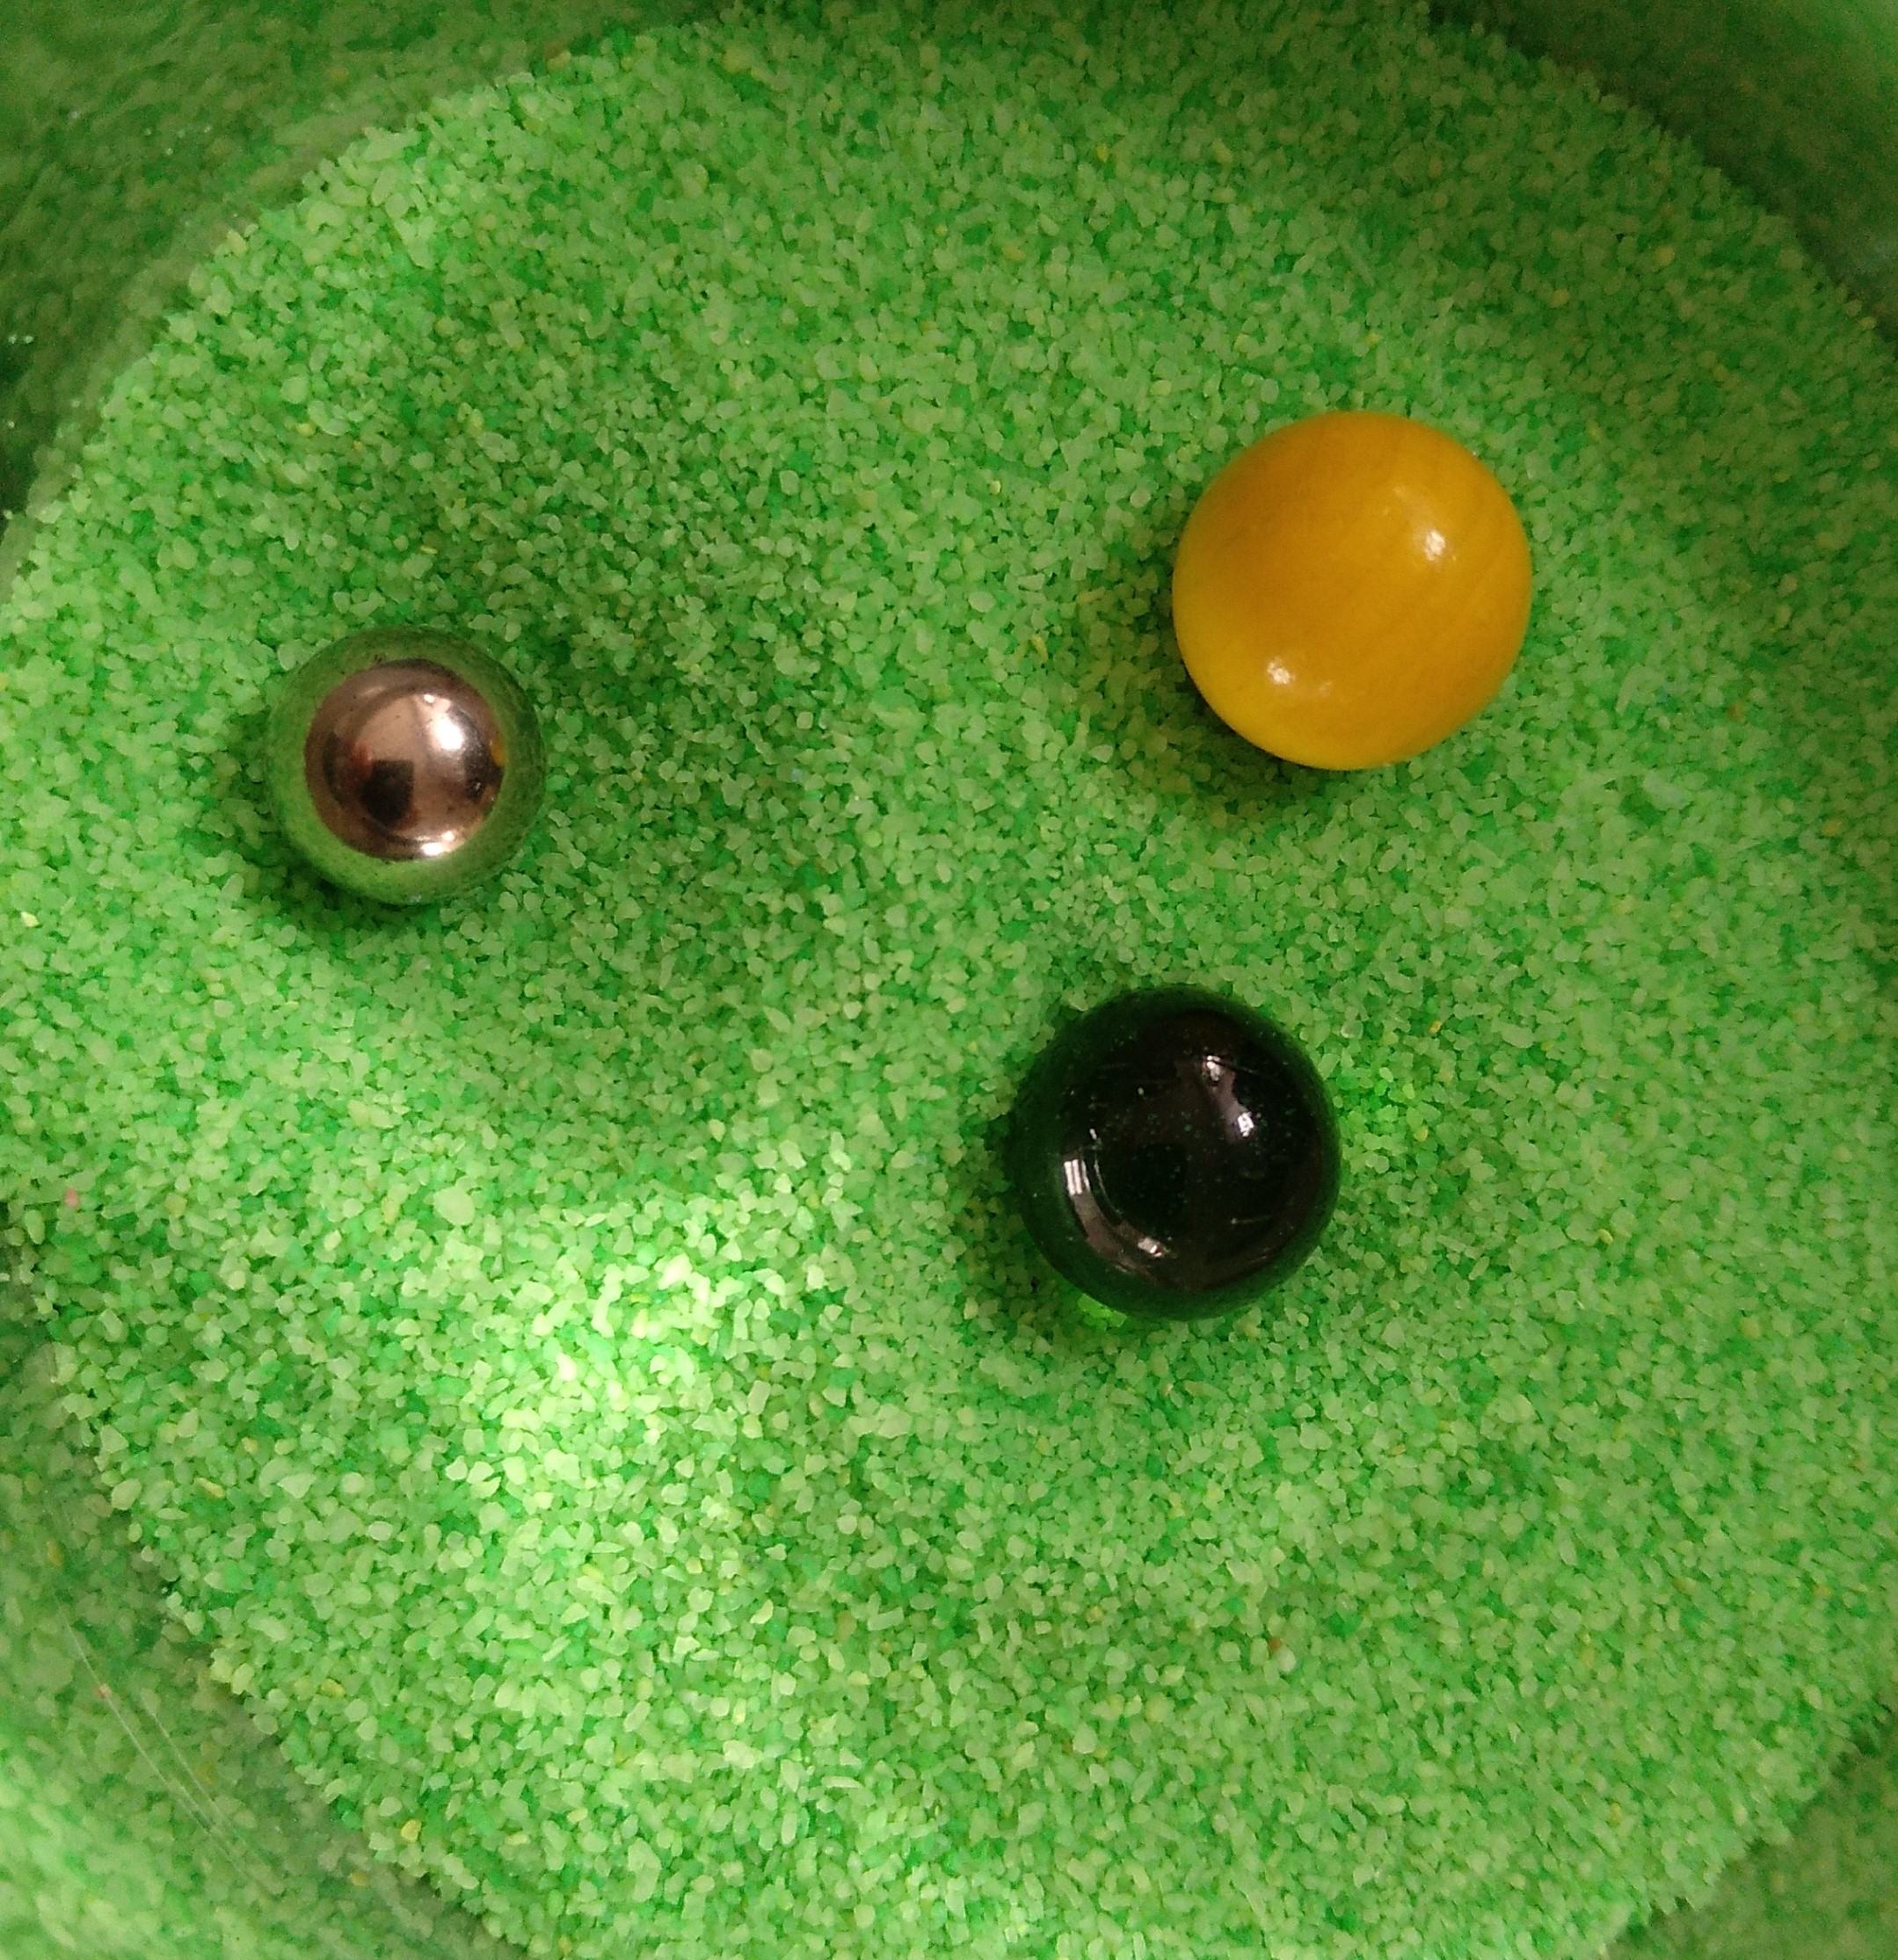
\includegraphics[width=0.5\textwidth]{Impuls}
	  \vspace{-3mm}
	  \caption{Bewegungsenergie fallender Kugeln}
   \end{figure}
}

\frame
{
  \frametitle{Kraftstoß und Impulsänderung}
\begin{align*}
F=m\cdot a=m\cdot\dfrac{\Delta v}{\Delta t}=\dfrac{v_t-v_0}{\Delta t}=\dfrac{\Delta p}{\Delta t}\\
v_0\quad\text{Geschwindigkeit vor der Impulsänderung}\\
v_t\quad\text{Geschwindigkeit nach der Impulsänderung}
\end{align*}
\begin{block}{Impulsänderung}
Der Kraftstoß entspricht der Änderung des Impulses eines bewegten Körpers.
\begin{align*}
\Delta p&=F\cdot \Delta t\\
\text{Kraftstoß}\quad I:\\
I=\Delta p&=F\cdot \Delta t=m\cdot v_t - m\cdot v_0
\end{align*}
\end{block}
}

\frame
{
  \frametitle{Simulation mit Algodoo}
      \begin{figure}
	  \includegraphics[width=0.8\textwidth]{Algodoo}
	  \vspace{-3mm}
	  \caption{Beispiel Impulsänderung}
   \end{figure}
}

\frame[allowframebreaks]
{
  \frametitle{Beispielaufgabe Impulsänderung}
  An einem Eisenbahnzug mit der Masse $m=\SI{960000}{\kilogram}$ wirkt eine Zugkraft $F_Z=\SI{120}{\kilo\newton}$.Die Gesamte Fahrwiderstandskraft (Reibung und Luftwiderstand) ist $F_F=\SI{47,1}{\kilo\newton}$. Berechnen Sie
\begin{enumerate}
\item die resultierende Kraft $F_r$,
\item $v_t$ nach $t=\SI{5}{\minute}$ (horizontale Strecke und $v_0=0$).
\end{enumerate}
\newpage
\textbf{Lösung:}\\
  \begin{tikzpicture}
  \begin{scope}[yscale=0.06, xscale=0.06]
  \begin{footnotesize}
    \draw[-latex, thick] (0,0) -- (47.1,0) node[midway, above] {$F_F$};
    \draw[latex-, thick] (0,14) -- (120,14) node[midway, above] {$F_Z=\text{Zugkraft}$};
	\draw[latex-, red, thick] (47.1,4) -- (120,4) node[midway, above] {$F_r=\text{Antriebskraft}$};
	\draw[thin] (0,-3) -- (0,17); 
	\draw[thin] (47.1,-3) -- (47.1,7);
	\draw[thin] (120,1) -- (120,17);
  \end{footnotesize}
  \end{scope}
  \end{tikzpicture}
\begin{enumerate}
\item Das Bild zeigt die zeichnerische Lösung. Danach ist:
	\begin{align*}
	F_r=F_Z-F_F=F_Z=\SI{120}{\kilo\newton}-F_F=\SI{47,1}{\kilo\newton}=F_F=\SI{72,9}{\kilo\newton}
	\end{align*}
\item 
	\begin{align*}
	F_{r} \cdot t&=m\cdot v_{t}-m\cdot v_{0}.\text{ Mit }v_0=0: F_r\cdot t=m\cdot v_{t}.\\
	\text{Somit: }v_t&=\dfrac{F_r\cdot t}{m}=\dfrac{\SI{72900}{\kilogram\meter\per\square\second}\cdot (5\cdot 60)\si{\second}}{\SI{960000}{\kilogram}}=\SI{22,78}{\meter\per\second}\\
	v_t&=\SI{82}{\kilo\meter\per\hour}
	\end{align*}
\end{enumerate}
}

\frame
{
  \frametitle{Impulserhaltung}
  \begin{block}{Impulserhaltungssatz}
  Ist die Summe aller äußeren am Körper angreifenden Kräfte Null, dann ändert sich der Impuls des Körpers nicht.
	\begin{align*}
	\textbf{Impulserhaltung}\quad\Delta p=0=m\cdot v_t-m\cdot v_0
	\end{align*}
  \end{block}
}

\frame[allowframebreaks]
{
  \frametitle{Der Stoß}
  \begin{tikzpicture}
  \begin{scope}[yscale=0.5, xscale=0.5]
  \begin{footnotesize}
  	\draw[thin] (0,0.25) -- (0,8);
  	\draw[thin] (1.5,0.75) -- (1.5,8);
  	\draw[thin] (-2,8) -- (3.5,8);
   	\fill[black] (0,8) circle (0.1);
   	\fill[black] (1.5,8) circle (0.1);
   	\fill[pattern=north east lines, very thin] (-2,8) -- (3.5,8) -- (3.5,8.5) -- (-2,8.5) -- cycle;
	\shadedraw[inner color=black!10!white,outer color=black!30!white, draw=black] (0,0) node {$m_1$} circle (0.5);
	\shadedraw[inner color=black!10!white,outer color=black!30!white, draw=black] (1.5,0) node {$m_2$} circle (1);
	\draw[latex-, very thick] (2.5,0) -- (6,0) node[midway, above] {$v_2$};
	\draw[latex-, very thick] (-2,0) -- (-0.5,0) node[midway, above] {$v_1$};
	\draw[thin, dashed] (0.5,-2.5) -- (0.5,2);
	\draw[latex-, very thick, red] (0.5,-2) -- (4.5,-2) node[midway, below] {$F_2=m_2\cdot a_2$};
	\draw[-latex, very thick, red] (-3.5,-2) -- (0.5,-2) node[midway, below] {$F_1=m_1\cdot a_1$};
  \end{footnotesize}
  \end{scope}
  \end{tikzpicture}
  \newpage
  	\begin{align*}
	F_1&=-F_2\\
	m_1\cdot a_1&=-m_2\cdot a_2\rightarrow m_1\cdot\dfrac{\Delta v_1}{\Delta t}=-m_2\cdot\dfrac{\Delta v_2}{\Delta t}\\
	\curvearrowright m_1\cdot\Delta v_1&=m_2\cdot\Delta v_2\rightarrow\dfrac{\Delta v_1}{\Delta v_2}=-\dfrac{m_2}{m_1}\\
	\end{align*}
	  \begin{block}{Stoß}
Die Geschwindigkeitsänderungen beim Stoß zweier Massen sind entgegengesetzt gerichtet und verhalten sich umgekehrt proportional zu den Massen.
  \end{block}
	  \begin{block}{Impulserhaltungssatz}
Beim Stoß ändert sich der Gesamtimpuls, d.h. die Summe aller Einzelimpulse in einem System bewegter Körper, nicht.
  \end{block}	
}

\frame
{
  \frametitle{Der unelastische Stoß}
  Beim unelastischen, d.h. plastischen Stoß verformt sich mindestens einer der beiden Körper vollkommen plastisch.
  \begin{block}{Geschwindigkeit beider Massen nach einem unelastischen Stoß}
	\begin{align*}
	v=\dfrac{m_1\cdot v_1+m_2\cdot v_2}{m_1+m_2}
	\end{align*}
  \end{block}
}

\frame
{
\uncover<1->
{
  \frametitle{Beispielaufgabe unelastischer Stoß}
Ein Körper mit der Masse $m_1=\SI{10}{\kilogram}$ bewegt sich mit $v_1=\SI{10}{\meter\per\second}$ auf einen Körper mit der Masse $m_2=\SI{100}{\kilogram}$, der sich in Ruhe befindet, zu. Wie groß ist die gemeinsame Endgeschwindigkeit $v$, wenn sich die Masse $m_1$ vollkommen plastisch verhält?
\includegraphics[width=0.3\textwidth]{unelastischer_Stoß.png}\\
}
\uncover<2->
{
\textbf{Lösung:}	
	\begin{align*}
	v&=\dfrac{m_1\cdot v_1+m_2\cdot v_2}{m_1+m_2}=\dfrac{\SI{10}{\kilogram}\cdot \SI{10}{\meter\per\second}+\SI{100}{\kilogram}\cdot 0}{\SI{10}{\kilogram}+\SI{100}{\kilogram}}=\dfrac{\SI{100}{\kilogram\meter\per\second}}{\SI{110}{\kilogram}}\\&=\SI{0,909}{\meter\per\second}
	\end{align*}
}
}

\frame
{
  \frametitle{Der elastische Stoß}
  Beim elastischen Stoß unterscheidet man den ersten Teil des Stoßes vom zweiten Teil des Stoßes.
  \begin{block}{Geschwindigkeit beider Massen nach der ersten Stoßhälfte}
	\begin{align*}
	\textbf{gemeinsame Geschwindigkeit: }v&=\dfrac{m_1\cdot v_1+m_2\cdot v_2}{m_1+m_2}\\
	\textbf{Endgeschwindigkeit }m_1:v_{1e}&=2\cdot\dfrac{m_1\cdot v_1+m_2\cdot v_2}{m_1+m_2}-v_1\\
	\textbf{Endgeschwindigkeit }m_2:v_{2e}&=2\cdot\dfrac{m_1\cdot v_1+m_2\cdot v_2}{m_1+m_2}-v_2\\
	\end{align*}
  \end{block}
}

\frame
{
  \frametitle{Beispielaufgabe elastischer Stoß}
Ein Körper mit der Masse $m_1=\SI{6}{\kilogram}$ bewegt sich mit $v_1=\SI{10}{\meter\per\second}$ zentrisch auf einen Körper mit der Masse $m_2=\SI{18}{\kilogram}$, der sich mit $v_2=\SI{2}{\meter\per\second}$ in die gleiche Richtung wie der Körper mit der Masse $m_1$ bewegt, zu. Berechnen Sie
\begin{enumerate}
\item Die Geschwindigkeit $v$ beider Körper nach der ersten Hälfte des Stoßes.
\item die Endgeschwindigkeiten beider Körper am Ende eines vollkommen elastischen Stoßes.
\end{enumerate}
}
\frame[allowframebreaks]
{
\textbf{Lösung:}	
\begin{enumerate}
\item 
	\begin{align*}
	v&=\dfrac{m_1\cdot v_1+m_2\cdot v_2}{m_1+m_2}=\dfrac{\SI{6}{\kilogram}\cdot \SI{10}{\meter\per\second}+\SI{18}{\kilogram}\cdot \SI{2}{\meter\per\second}}{\SI{6}{\kilogram}+\SI{18}{\kilogram}}=\dfrac{\SI{96}{\kilogram\meter\per\second}}{\SI{24}{\kilogram}}\\
	&=\SI{4}{\meter\per\second}
	\end{align*}
\item 
	\begin{align*}
	v_{1e}&=2\cdot\dfrac{m_1\cdot v_1+m_2\cdot v_2}{m_1+m_2}-v_1\\
	&=2\cdot\dfrac{\SI{6}{\kilogram}\cdot \SI{10}{\meter\per\second}+\SI{18}{\kilogram}\cdot \SI{2}{\meter\per\second}}{\SI{6}{\kilogram}+\SI{18}{\kilogram}}-\SI{10}{\meter\per\second}=\SI{8}{\meter\per\second}-\SI{10}{\meter\per\second}\\
	&=-\SI{2}{\meter\per\second}\\
		v_{2e}&=2\cdot\dfrac{m_1\cdot v_1+m_2\cdot v_2}{m_1+m_2}-v_2\\
	&=2\cdot\dfrac{\SI{6}{\kilogram}\cdot \SI{10}{\meter\per\second}+\SI{18}{\kilogram}\cdot \SI{2}{\meter\per\second}}{\SI{6}{\kilogram}+\SI{18}{\kilogram}}-\SI{2}{\meter\per\second}=\SI{8}{\meter\per\second}-\SI{2}{\meter\per\second}\\
	&=\SI{6}{\meter\per\second}
	\end{align*}
\end{enumerate}
}

\frame
{
  \frametitle{Überblick über Begriffe der Mechanik}
\begin{block}{Beschreibung}
\vspace{0.5cm}
% \usepackage{array} is required
\begin{tabular}{|>{\centering\arraybackslash}p{3cm}|>{\centering\arraybackslash}p{3cm}|>{\centering\arraybackslash}p{3cm}|}
\hline
\rule[-1ex]{0pt}{2.5ex} Energie & Kraft & Arbeit \\
\hline 
\rule[-1ex]{0pt}{2.5ex} Leistung & Potential & Feld \\ 
\hline 
\end{tabular}
\vspace{0.5cm}
\end{block}
Am Beispiel der schiefen Ebene.
}

\frame
{
  \frametitle{Energie}
\begin{block}{Beschreibung}
Unter Energie versteht man gespeicherte Arbeit, d.h. Fähigkeit eines Systems, Arbeit zu verrichten. Energie kann zwischen verschiedenen Energieformen hin- und her gewandelt werden, aber die Gesamtenergie bleibt dabei erhalten (Energieerhaltungssatz).
\end{block}
Die SI-Einheit der Energie $E$ ist:
$[E]=\SI{1}{\newton\meter}=\SI{1}{\joule}=\SI{1}{\kilo\gram\square\meter\per\square\second}$
      \begin{figure}
	  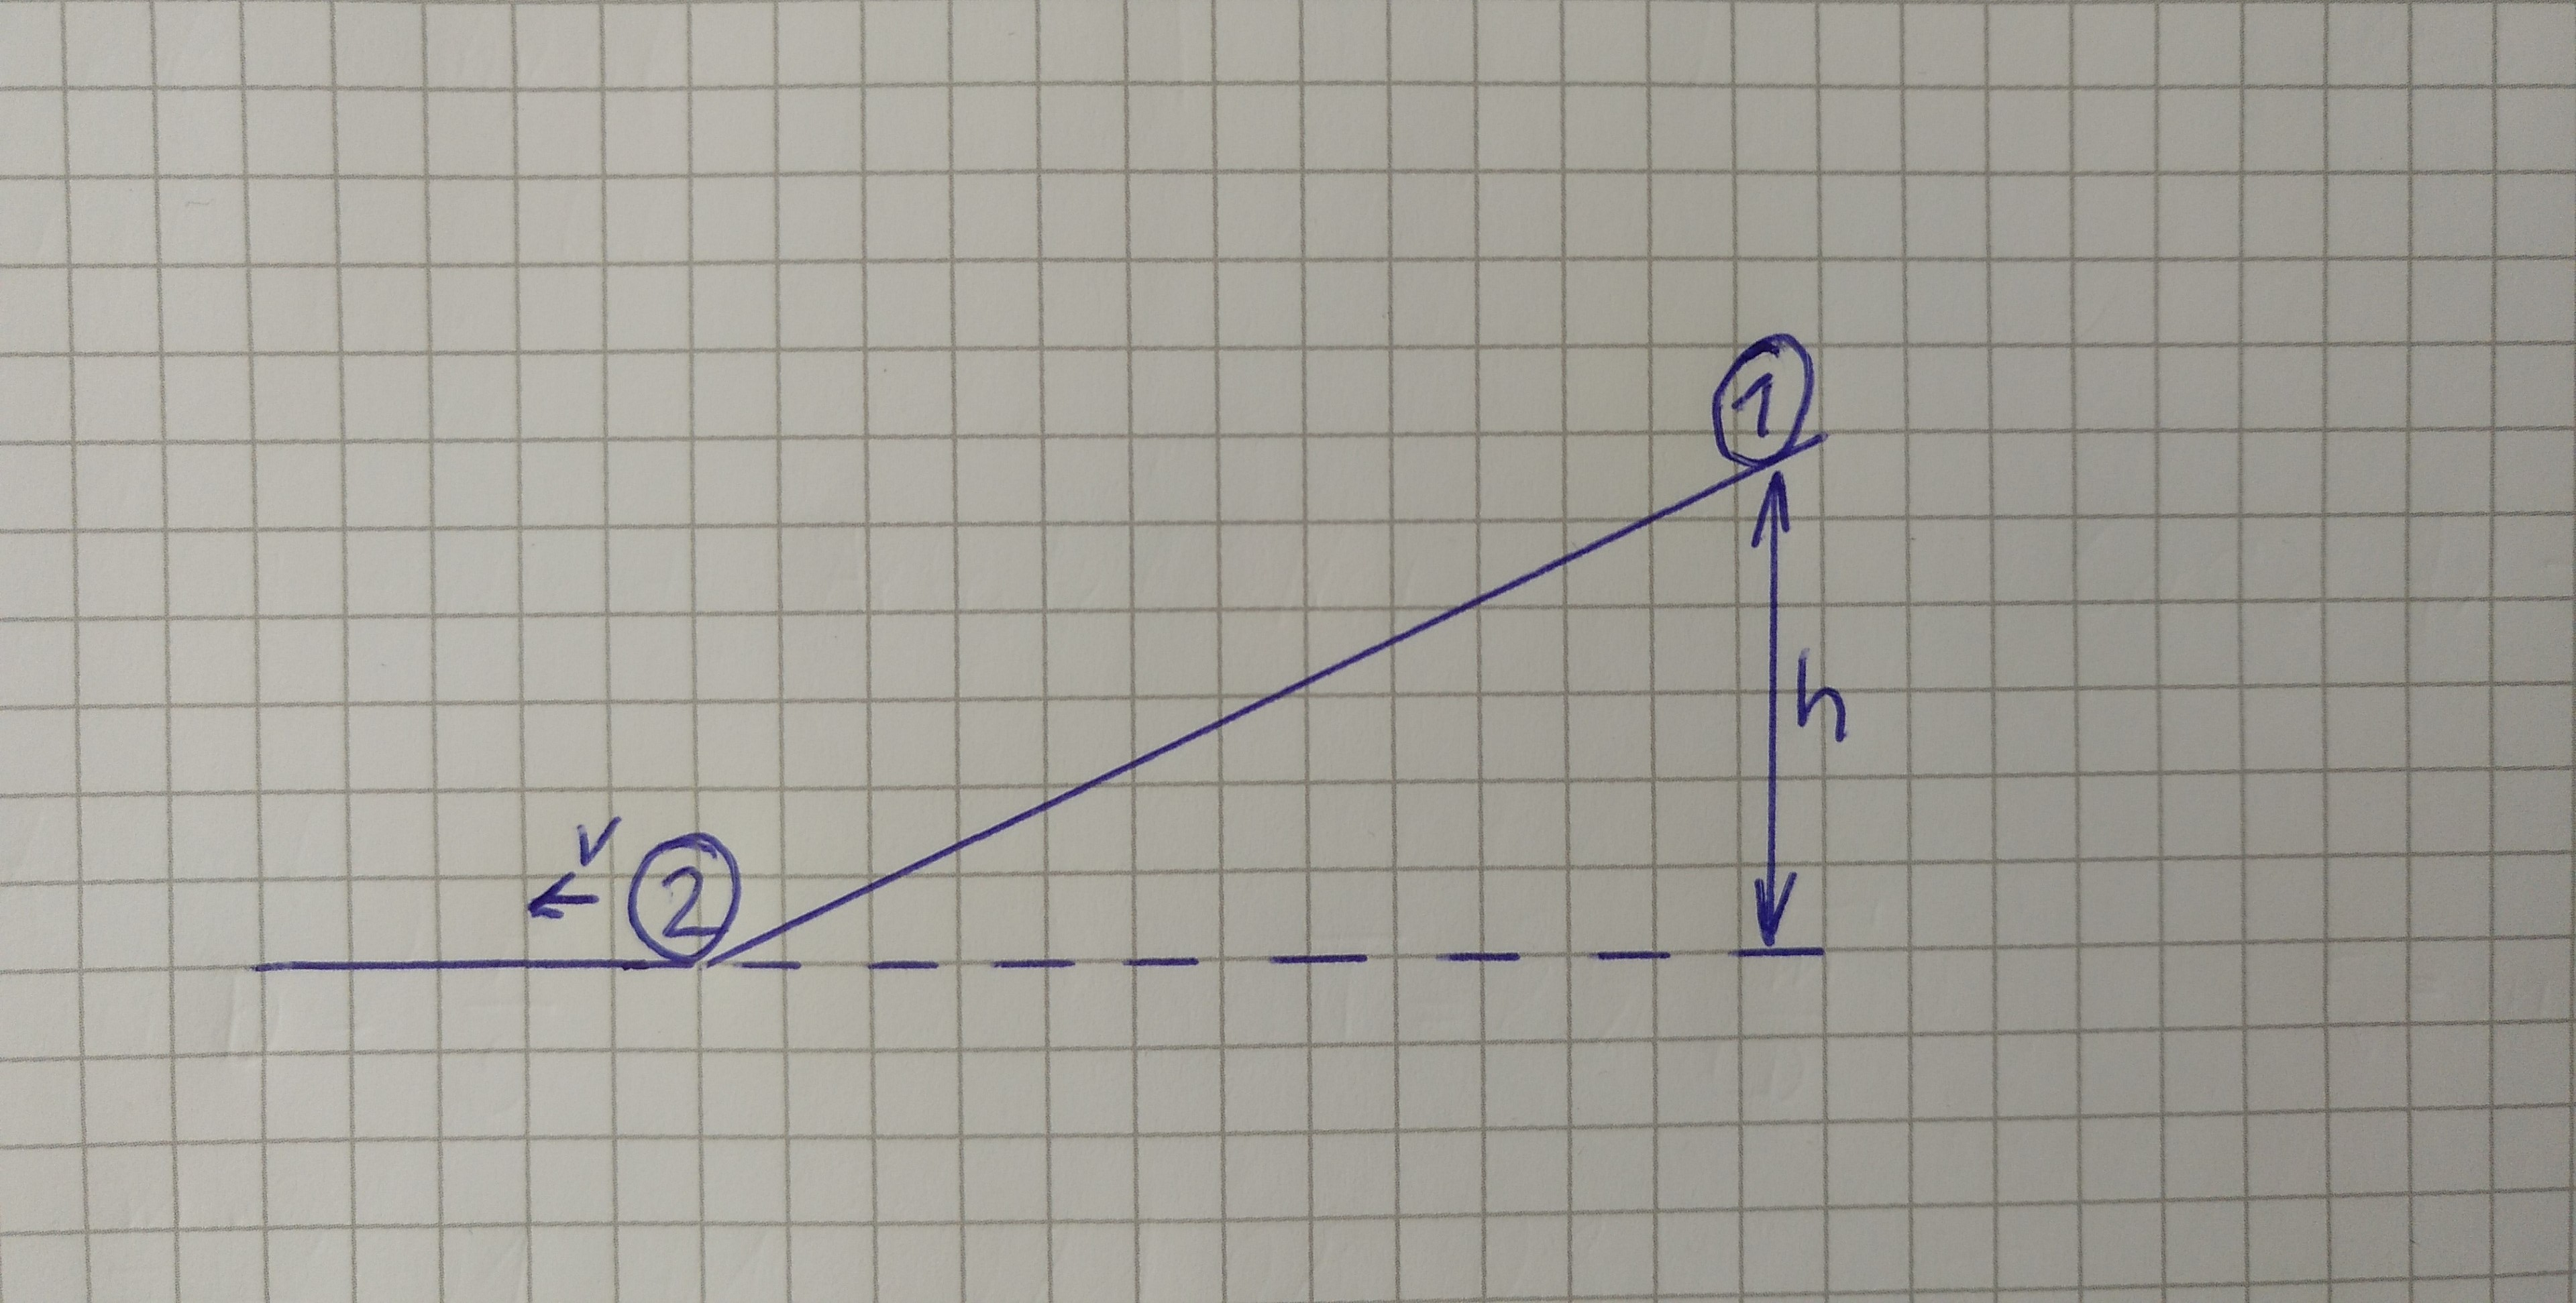
\includegraphics[width=0.8\textwidth]{Energie_1}
	  \vspace{-3mm}
	  \caption{Energie an der schiefen Ebene}
   \end{figure}
}

\frame
{
  \frametitle{Kraft}
\begin{block}{Beschreibung}
Eine Kraft ist durch ihre Größe (Stärke), ihre Richtung und ihren Angriffspunkt eindeutig bestimmt. Sie kann Körper verformen oder beschleunigen.
\end{block}
Die SI-Einheit der Kraft $F$ ist:
$[F]=\SI{1}{\newton}=\SI{1}{\kilo\gram\meter\per\square\second}$
      \begin{figure}
	  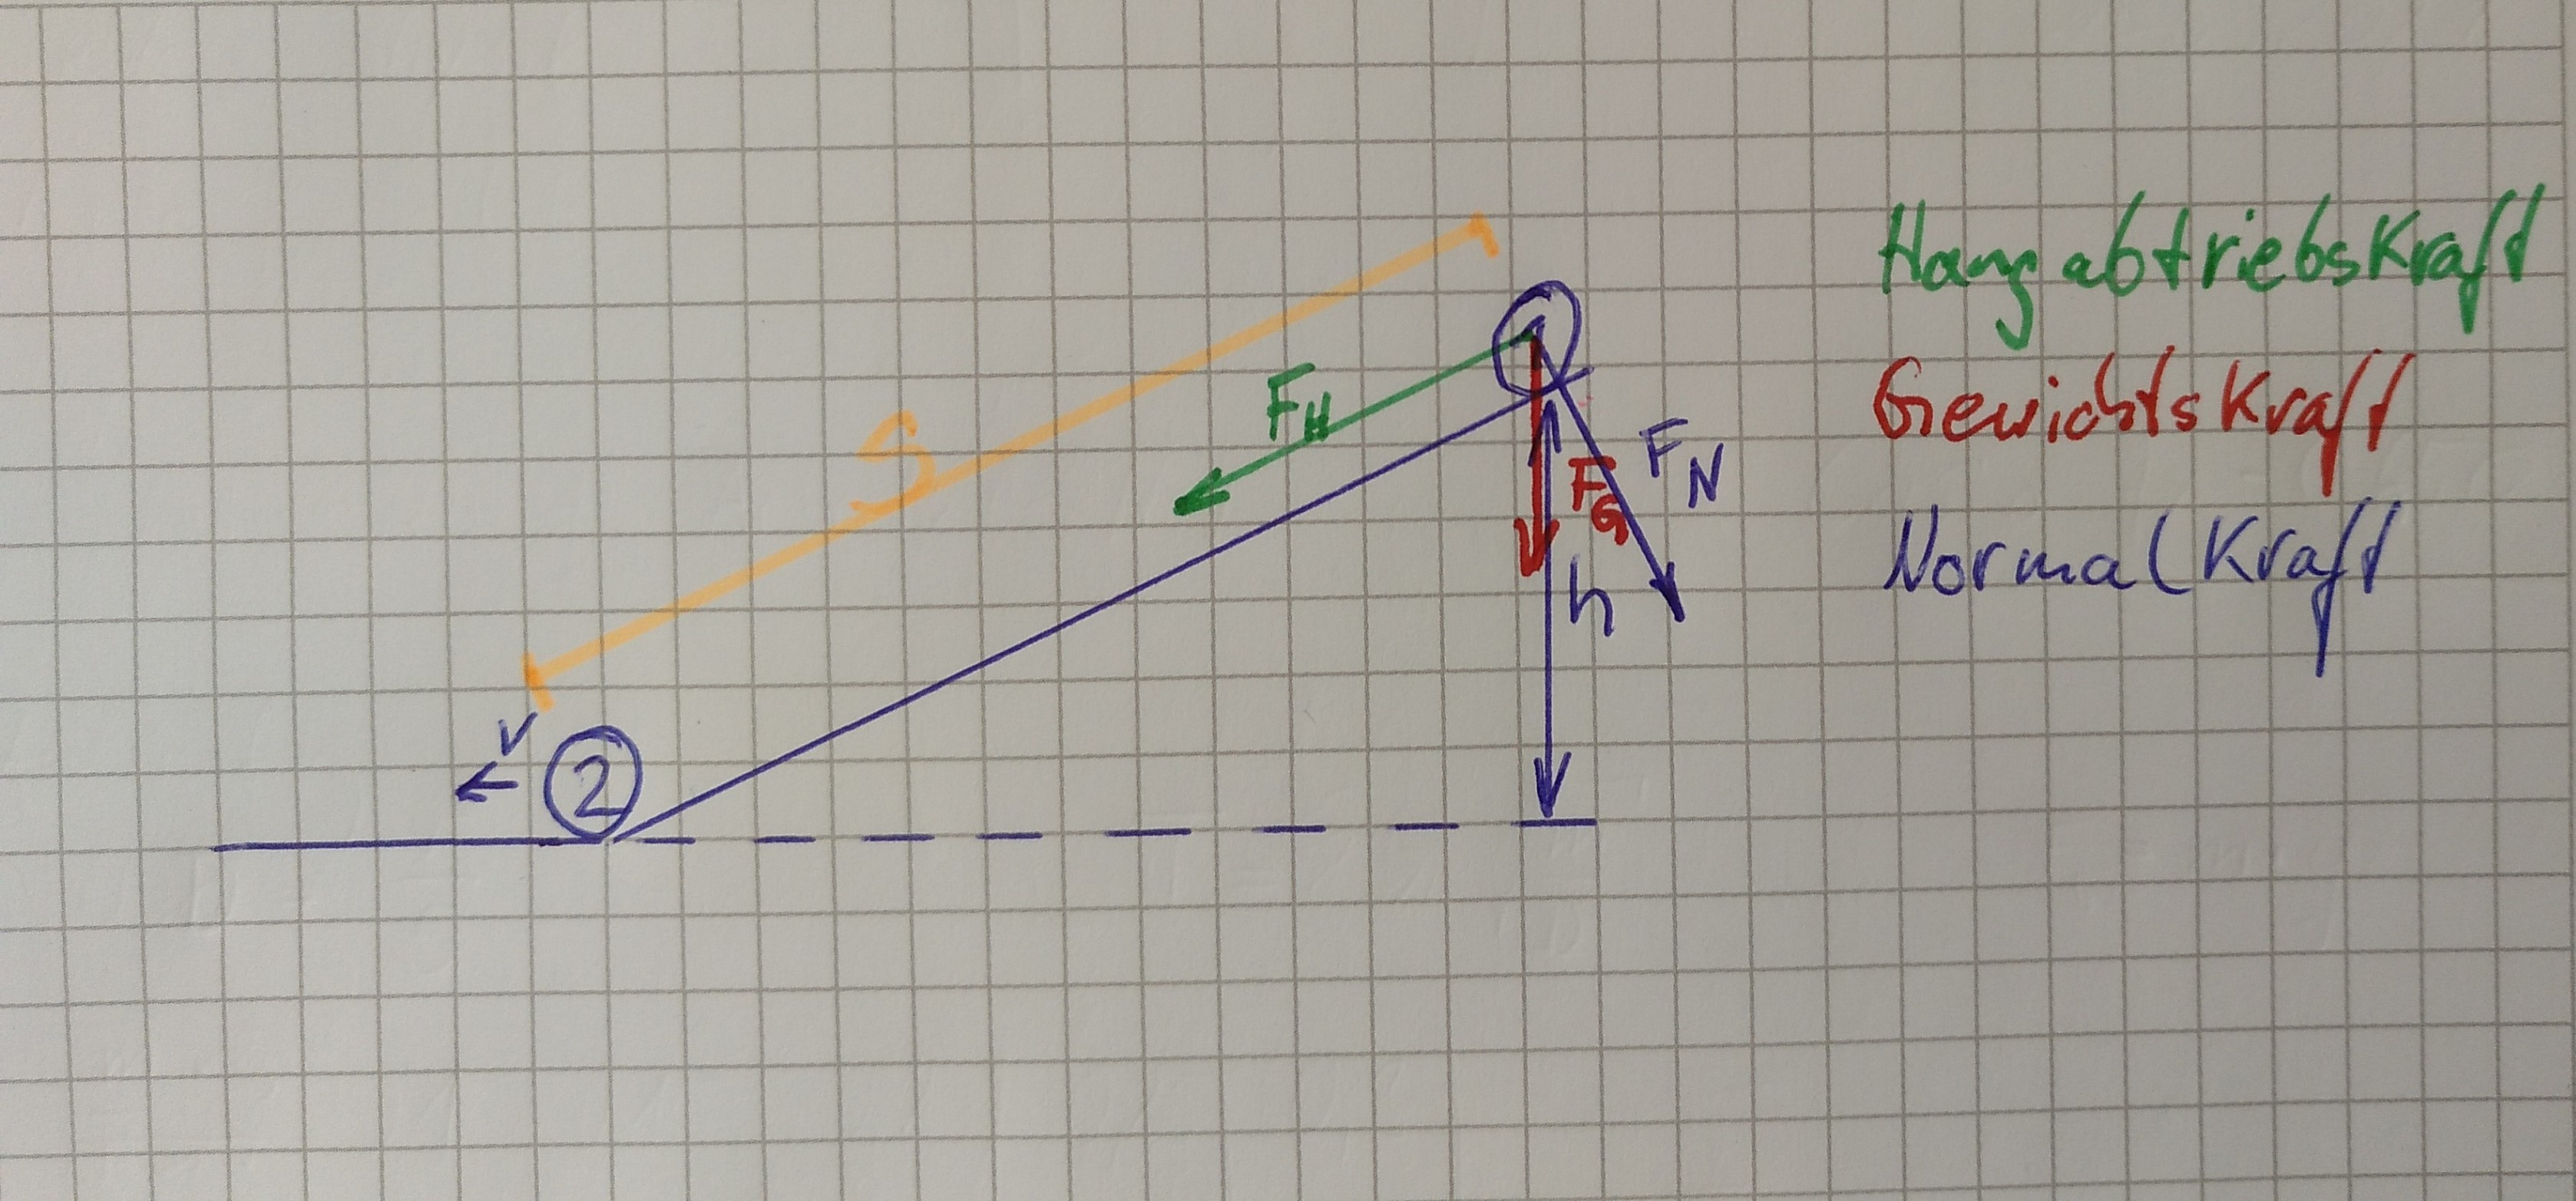
\includegraphics[width=0.8\textwidth]{Kraft}
	  \vspace{-3mm}
	  \caption{Kräfte an der schiefen Ebene}
   \end{figure}
     Wirkt die Kraft entlang eines Weges, so kann sie Energie übertragen bzw. Arbeit verrichten.
}

\frame
{
  \frametitle{Arbeit}
\begin{block}{Beschreibung}
Arbeit ist das Produkt aus der wirkenden Kraft $F$ und dem zurückgelegten Weg $s$ des bewegten Körpers. Durch Arbeit kann Energie in eine andere Form gewandelt werden.
\end{block}
Die SI-Einheit der Arbeit $W$ ist:
$[W]=\SI{1}{\newton\meter}=\SI{1}{\kilo\gram\square\meter\per\square\second}=\SI{1}{\joule}$
      \begin{figure}
	  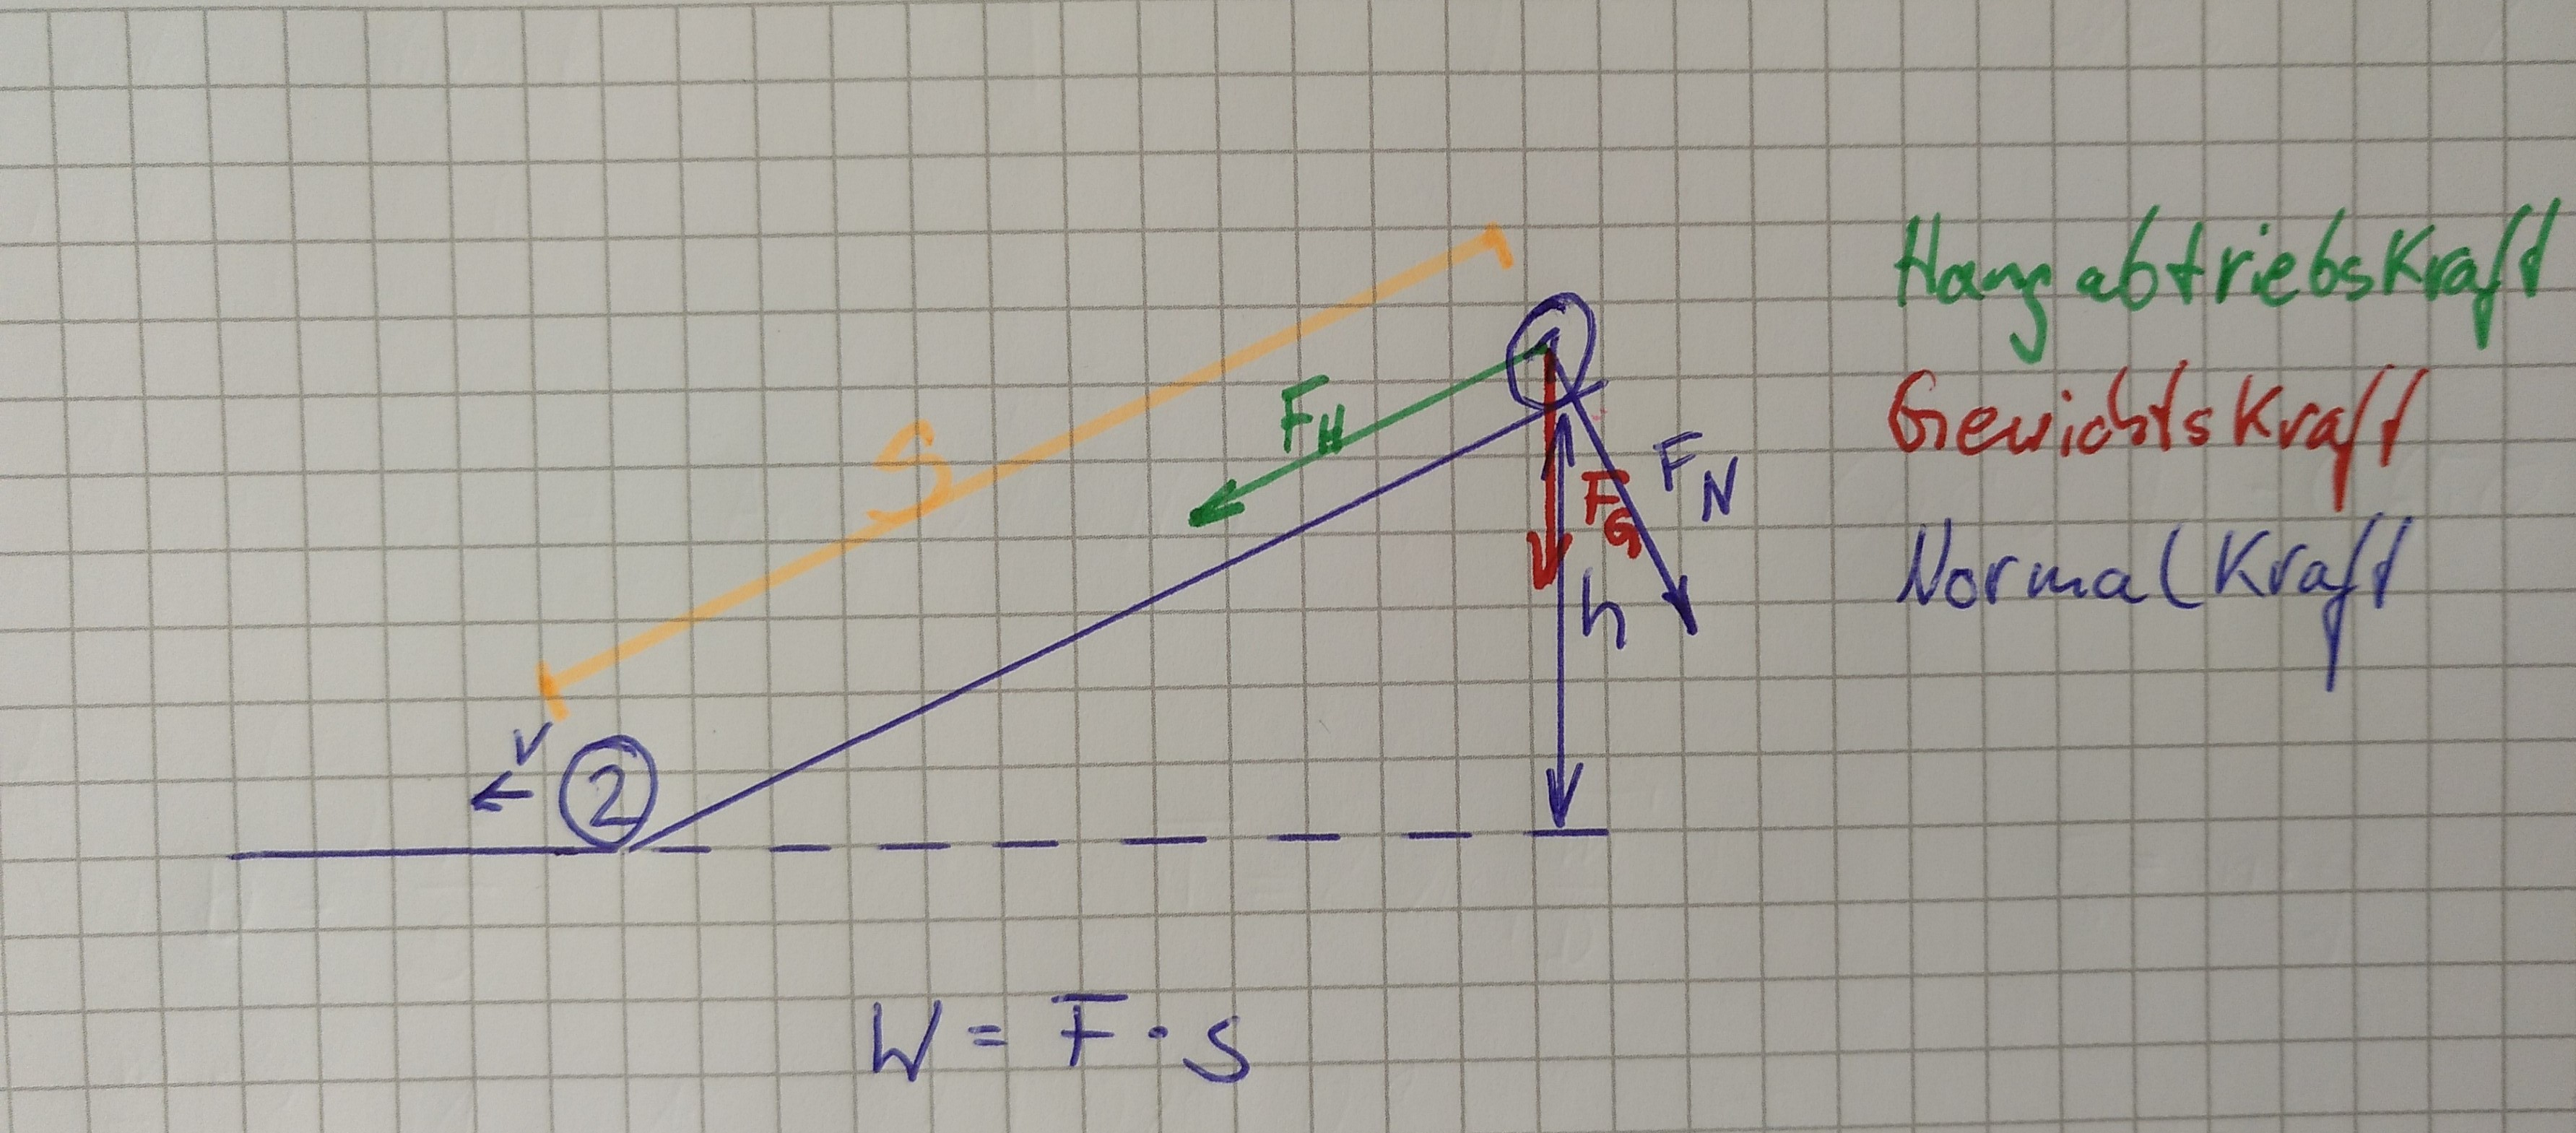
\includegraphics[width=0.8\textwidth]{Arbeit_1}
	  \vspace{-3mm}
	  \caption{Arbeit an der schiefen Ebene}
   \end{figure}
}

\frame
{
  \frametitle{Leistung}
\begin{block}{Beschreibung}
Die mechanische Leistung ist gleich dem Quotienten aus der mechanischen Arbeit und der für die Verrichtung dieser Arbeit erforderlichen Zeit. Sie gibt an, in welchem Maß ein System Arbeit verrichten kann.
\end{block}
SI-Einheit der Leistung $P$:
$[P]=\SI{1}{\newton\meter\per\second}=\SI{1}{\joule\per\second}=\SI{1}{\kilo\gram\square\meter\per\cubic\second}=\SI{1}{\watt}$
      \begin{figure}
	  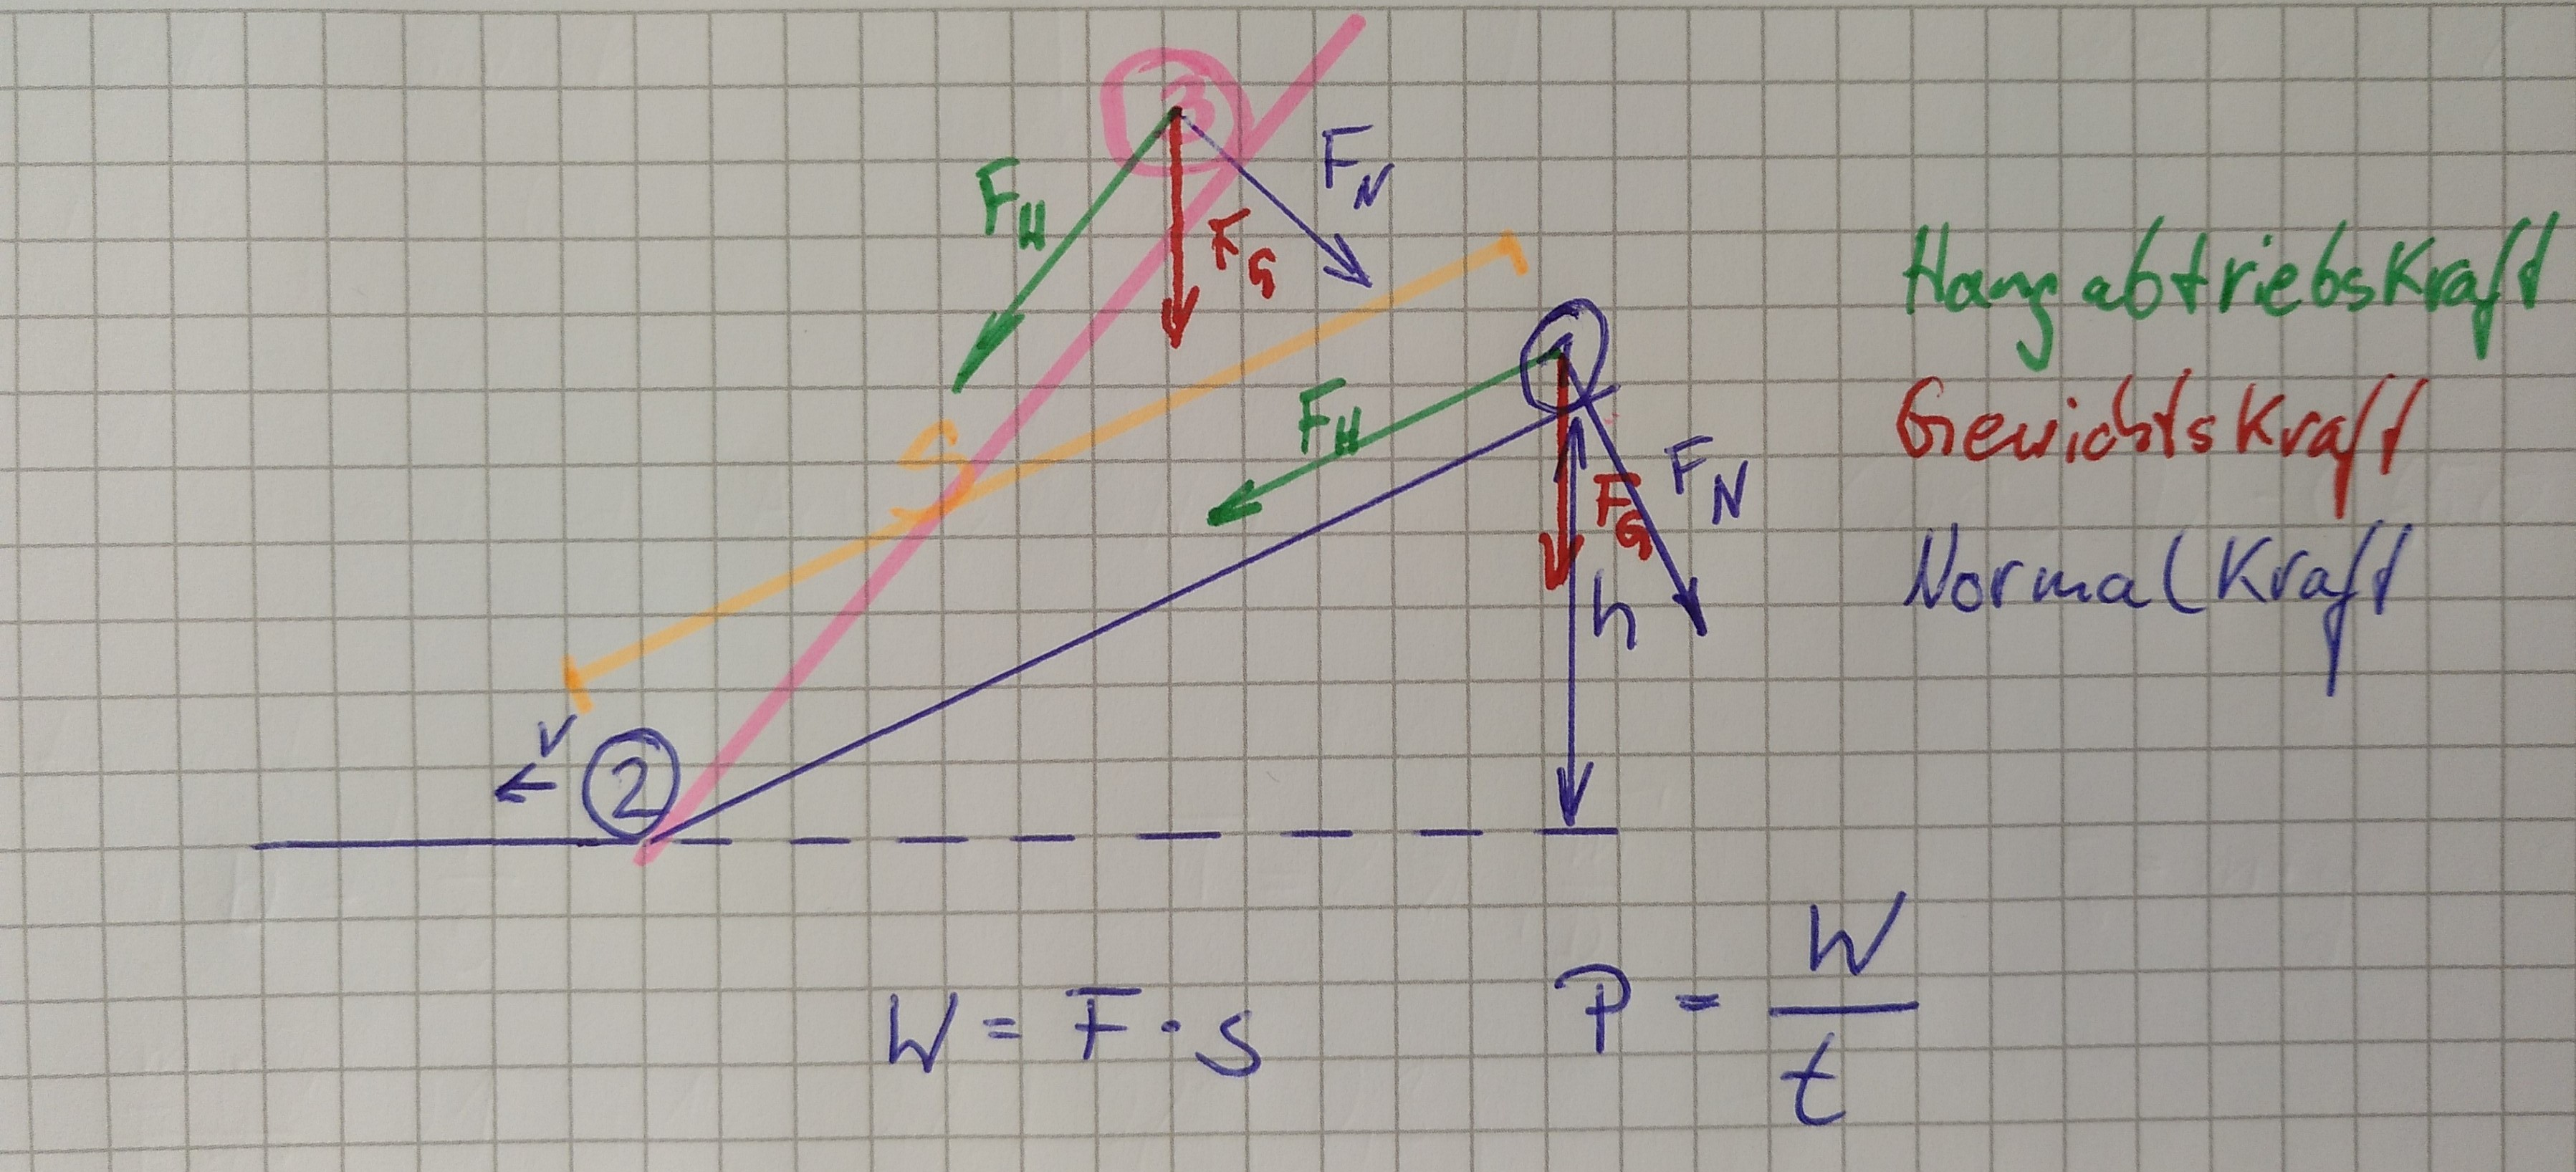
\includegraphics[width=0.6\textwidth]{Leistung}
	  \vspace{-3mm}
	  \caption{Leistung an der schiefen Ebene}
   \end{figure}
   Je mehr Energie ein System pro Sekunde umwandeln kann, desto größer ist seine Leistung.
}

\frame
{
  \frametitle{Potential}
\begin{block}{Beschreibung}
Das Potential, das ein Körper in einem Feld hat, beschreibt, wie viel Arbeit das Feld an ihm verrichten kann. Das Potential hängt vom gewählten Bezugspunkt ab.
\end{block}
      \begin{figure}
	  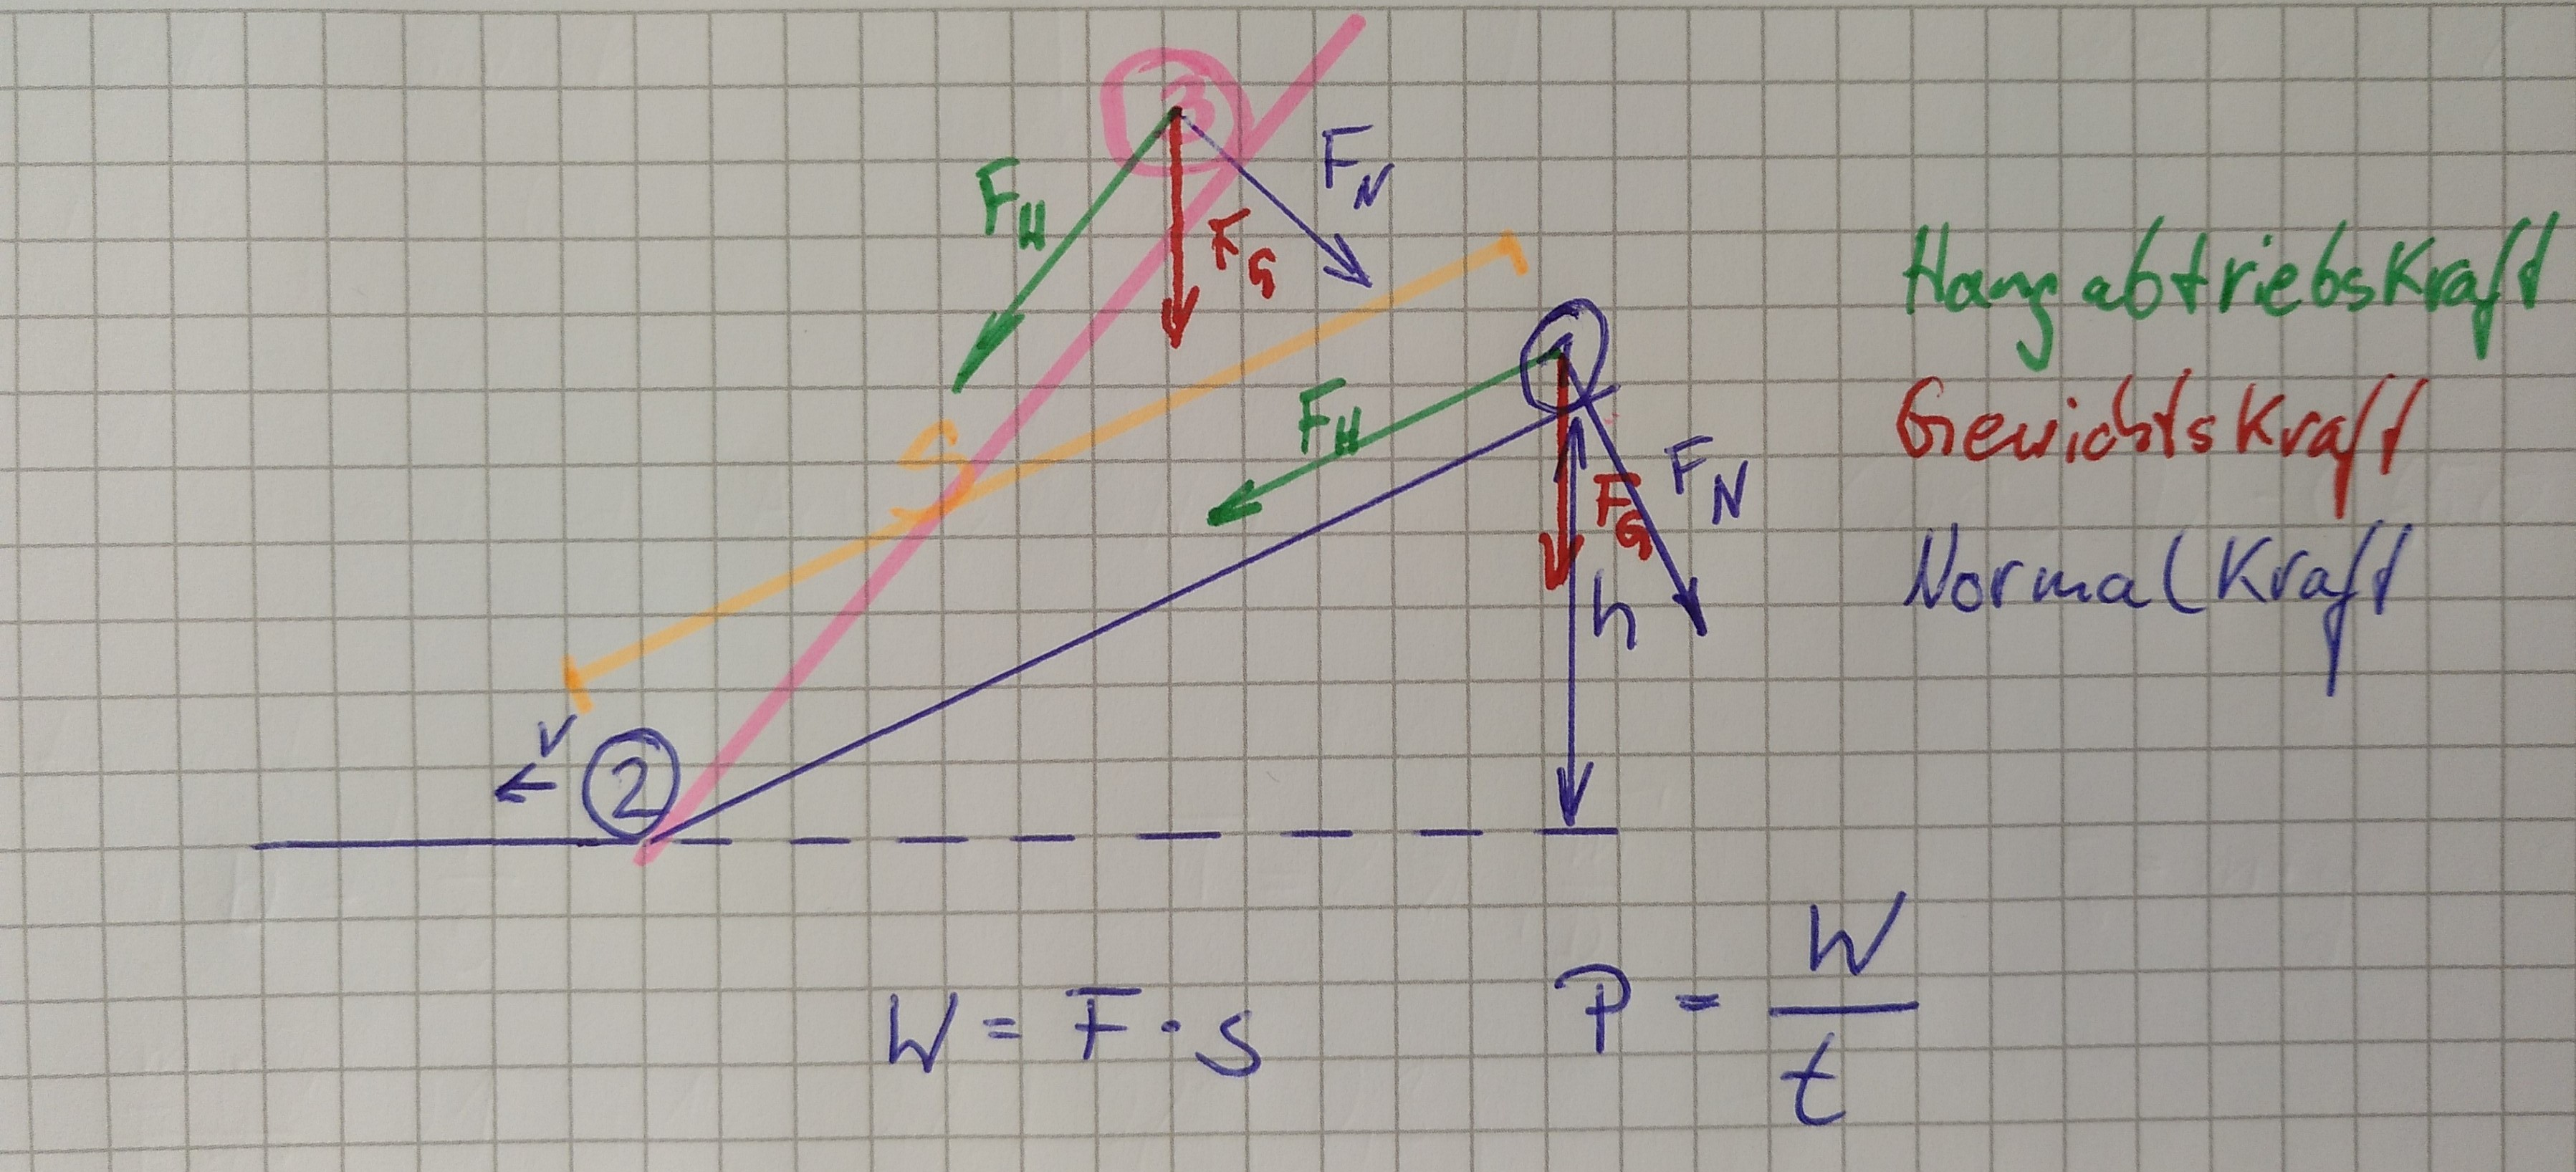
\includegraphics[width=0.75\textwidth]{Leistung}
	  \vspace{-3mm}
	  \caption{Potential an der schiefen Ebene}
   \end{figure}
}

\frame
{
  \frametitle{Feld}
\begin{block}{Beschreibung}
Ein "Feld" nennt man einen Bereich im Raum, in dem auf einen Körper eine Kraft wirkt. z.B. das Gravitationsfeld der Erde.
\end{block}
      \begin{figure}
	  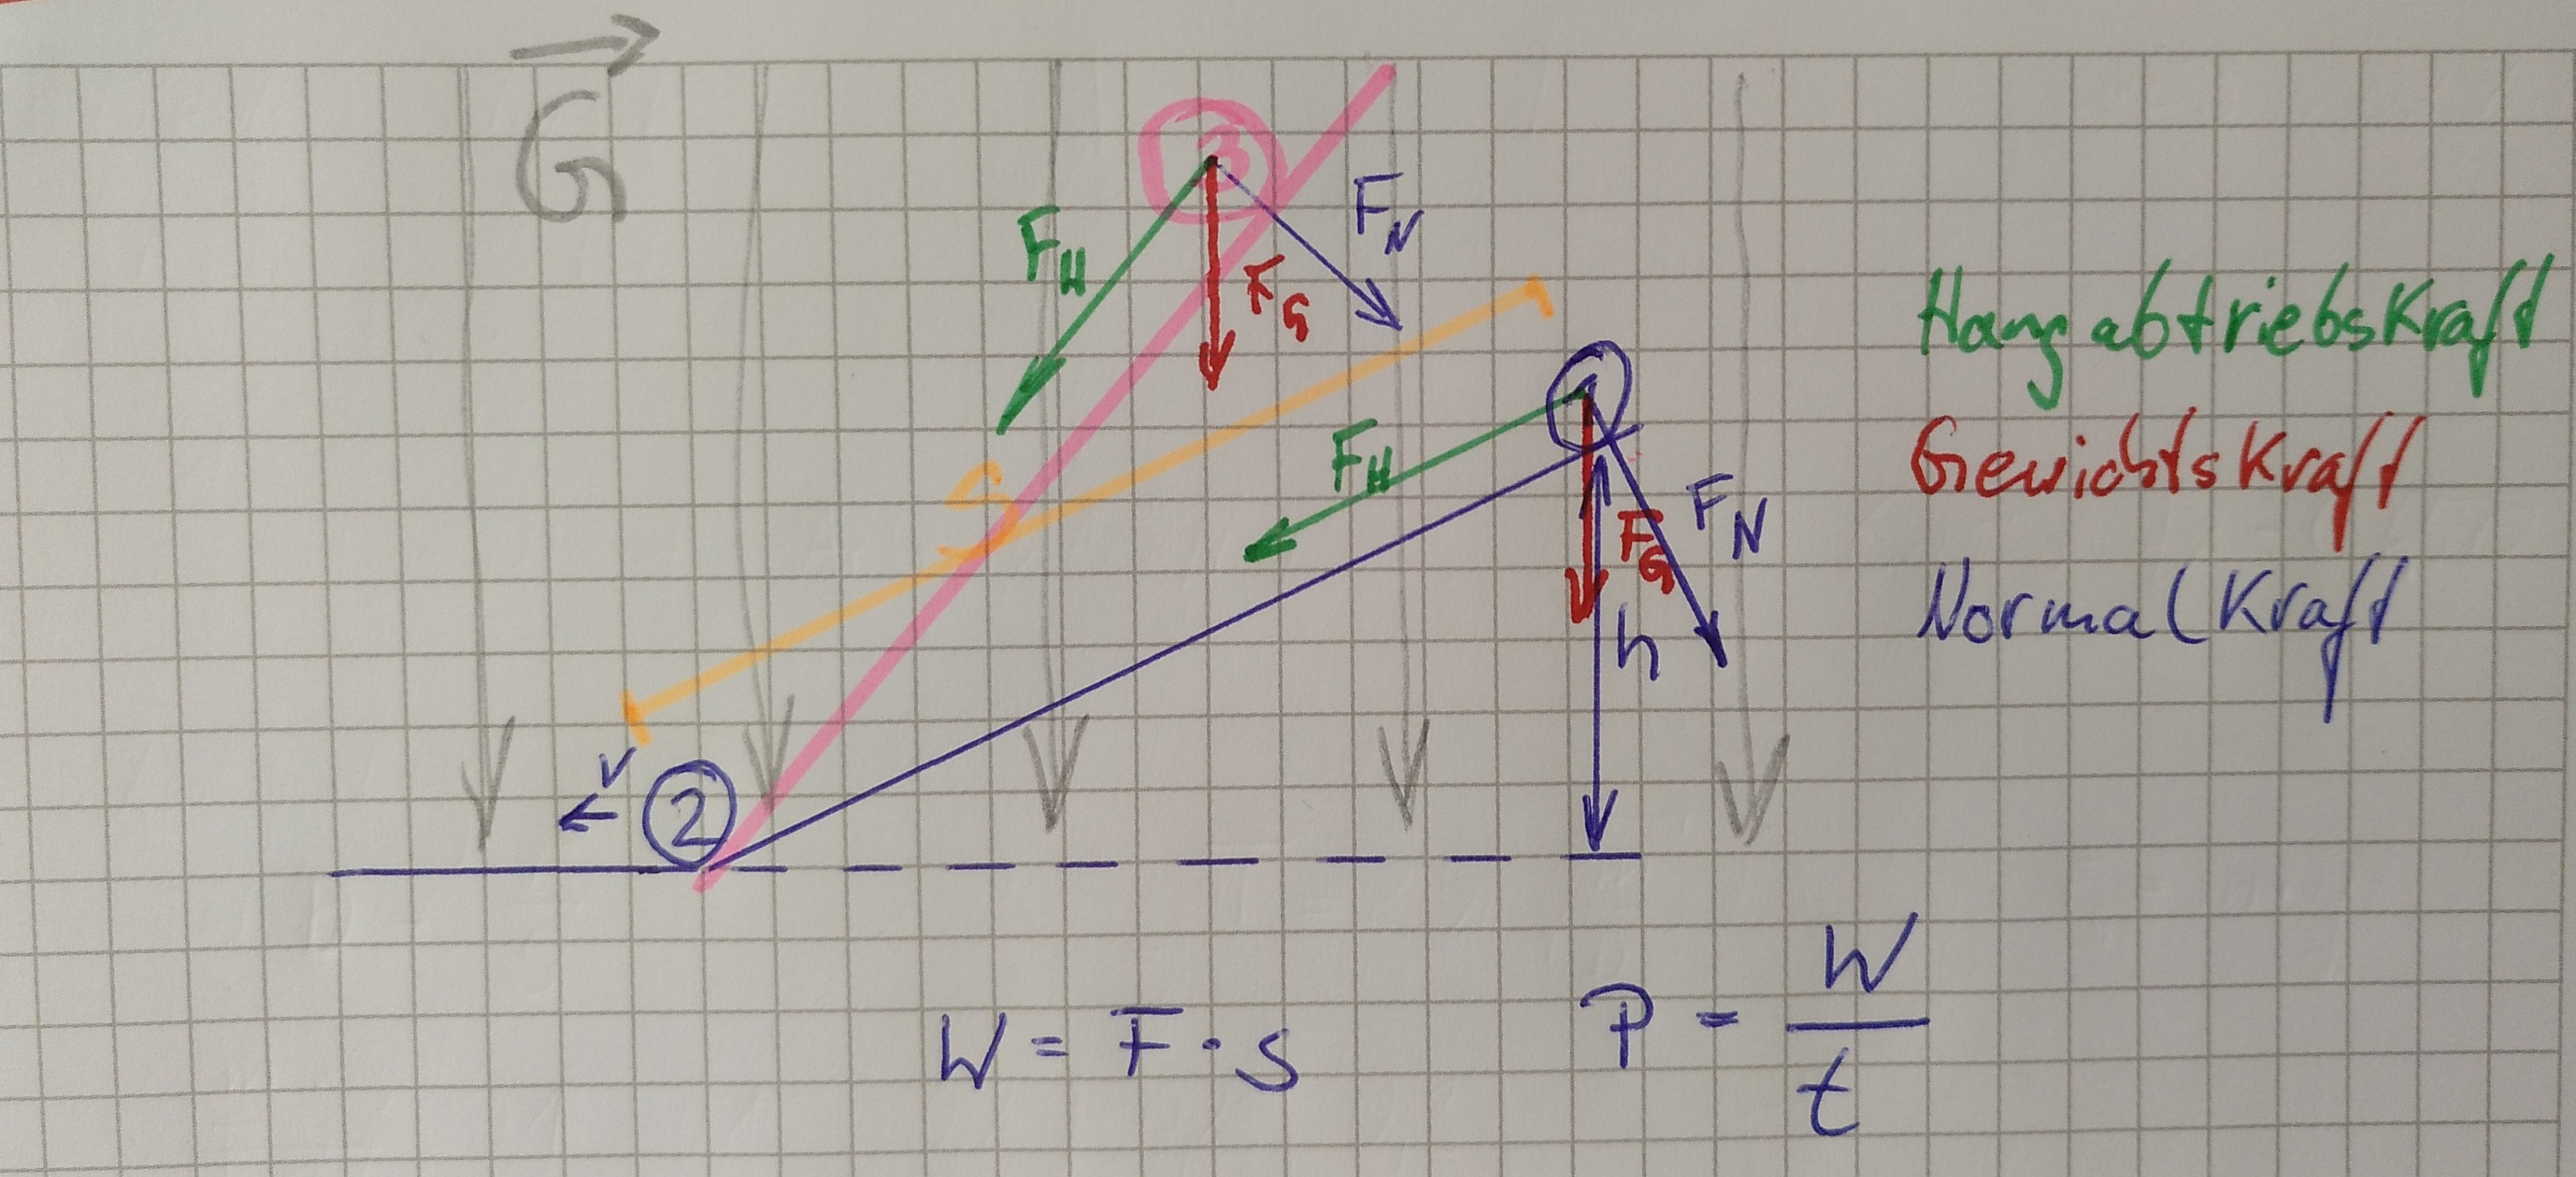
\includegraphics[width=0.8\textwidth]{Feld}
	  \vspace{-3mm}
	  \caption{Gravitationsfeld an der schiefen Ebene}
   \end{figure}
}
\end{document}
